\documentclass[paper=a4, fontsize=11pt]{scrartcl} % A4 paper and 11pt font size
\usepackage[utf8]{inputenc}
\usepackage[T1]{fontenc} % Use 8-bit encoding that has 256 glyphs
\usepackage[norsk]{babel} % English language/hyphenation
\usepackage{amsmath,amsfonts,amsthm} % Math packages

\usepackage{graphicx}
\usepackage{siunitx}

\usepackage[nottoc]{tocbibind}

\usepackage{sectsty} % Allows customizing section commands
\allsectionsfont{\centering \normalfont\scshape} % Make all sections centered, the default font and small caps

\usepackage{fancyhdr} % Custom headers and footers
\pagestyle{fancyplain} % Makes all pages in the document conform to the custom headers and footers
\fancyhead[L]{GRUPPE 1} % No page header - if you want one, create it in the same way as the footers below
\fancyfoot[L]{} % Empty left footer
\fancyfoot[C]{} % Empty center footer
\fancyfoot[R]{\thepage} % Page numbering for right footer
\renewcommand{\headrulewidth}{0pt} % Remove header underlines
\renewcommand{\footrulewidth}{0pt} % Remove footer underlines
\setlength{\headheight}{13.6pt} % Customize the height of the header

\usepackage{hyperref}
\hypersetup{
    colorlinks,
    citecolor=black,
    filecolor=black,
    linkcolor=black,
    urlcolor=black
}

\fancypagestyle{firststyle}
{
  \fancyhf{}
  \fancyfoot[R]{\thepage}
}

\numberwithin{equation}{section} % Number equations within sections (i.e. 1.1, 1.2, 2.1, 2.2 instead of 1, 2, 3, 4)
\numberwithin{figure}{section} % Number figures within sections (i.e. 1.1, 1.2, 2.1, 2.2 instead of 1, 2, 3, 4)
\numberwithin{table}{section} % Number tables within sections (i.e. 1.1, 1.2, 2.1, 2.2 instead of 1, 2, 3, 4)

\newcounter{alphasect}
\def\alphainsection{0}

\let\oldsection=\section
\def\section{%
  \ifnum\alphainsection=1%
    \addtocounter{alphasect}{1}
  \fi%
\oldsection}%

\renewcommand\thesection{%
  \ifnum\alphainsection=1% 
    \Alph{alphasect}%
  \else
    \arabic{section}%
  \fi%
}%

\newenvironment{alphasection}{%
  \ifnum\alphainsection=1%
    \errhelp={Let other blocks end at the beginning of the next block.}
    \errmessage{Nested Alpha section not allowed}
  \fi%
  \setcounter{alphasect}{0}
  \def\alphainsection{1}
}{%
  \setcounter{alphasect}{0}
  \def\alphainsection{0}
}%


%----------------------------------------------------------------------------------------
%   TITLE SECTION
%----------------------------------------------------------------------------------------

\newcommand{\horrule}[1]{\rule{\linewidth}{#1}} % Create horizontal rule command with 1 argument of height

\title{ 
\normalfont \normalsize 
\textsc{Norwegian University of Science and Technology} \\ [25pt] % Your university, school and/or department name(s)
\horrule{0.5pt} \\[0.4cm] % Thin top horizontal rule
\huge \textbf{Øving 1} \\ % The assignment title
TIØ4258 \\
\horrule{2pt} \\[0.5cm] % Thick bottom horizontal rule
}

\author{GRUPPE 1:\\Iver Jordal\\Stian Jensen\\Christian Tverås\\Asbjørn Ottesen Steinskog\\Julie Johnsen Kirkhus\\Christoffer Tønnessen}

\date{\normalsize \today}

\begin{document}


\pagenumbering{roman}

\maketitle

\thispagestyle{firststyle}

\newpage

\renewcommand*\contentsname{Innhold}
\tableofcontents

\setcounter{secnumdepth}{3}

\newpage

\pagenumbering{arabic}

\section{Oppgave 1}
%Oppgave 1: Innovasjon og organisasjonsstruktur 

\subsection{Eksempler på to organiseringsformer}

\subsubsection{Norsk Radiokontroll AS}

% delkapittel II og III fra Case NoRAS er mest relevant

Norsk Radiokontroll AS produserer RC-løsninger til industriformål.

Bedriften har to produksjonsavdelinger, én som står for mikrokontrollsystemene, og én som tar seg av plaststøping av styringsenheter.

Radio- og elektronikkomponenter er standard, og kjøpes inn fra eksterne produsenter.

De har også en egen markedsføringsenhet som besøker kunder.

Det er nærliggende å si at bedriften er organisert med en funksjonell struktur.
De to produksjonsavdelingene arbeider på hver sin del av det samme produktet, inndelt etter om de jobber med plaststøping eller mikrokontrollere.

Endring av bedriften:

Noen mener lederstilen er bra, problemet er at teknisk kvalitet er for dårlig.
Flere kunder har antydet dette.

De andre mener problemet er lederstilen til Elisabeth.
Hun er for teknisk opptatt, og detaljstyrer for mye.
Dette går utover hennes til overordnet styring av bedriften.

Plan etter møte:
Ansatte ekspert på salg for å avlaste Elisabeth.
Utvide kompetanse på mikrosystemer
Opprette egen teknisk dokumentasjons-avdeling.

I april 1996 slår bedriften seg sammen med en plastbedrift fra Horten, Industriplast.
Noen måneder etter sammenslåingen ble de tre eierne av bedriften enige om å omstrukturere selskapet. Olav Heier, den tidligere sjefen fra Industriplast tok over som konsernsjef, slik at Elisabeth kunne tre over i en stilling som teknisk direktør.


\subsubsection{STOL AS}
% kanskje stol AS?

Nettverksstruktur:

Mekk og bøy, avtale om leveranse av metalldeler til stolene.
Leverandør av ull, både ULLSPESIALISTEN og TYNSET-GARN.
Skinn - kortere kontrakter (tre måneder).
Samarbeid med SENG AS om å levere en bredere produktlinje (stoler, soveromsmøbler).

70-tallet var en periode med mange omorganiseringer, hvor de gikk fra avtale med to ull-leverandører til å kjøpe opp den ene av dem.

\subsection{Fordeler og ulemper med organiseringsmodellene}

\subsubsection{Norsk Radiokontroll AS}


\subsubsection{STOL AS}

Fordeler med å ha virksomheten distribuert utover flere firmaer er at de ulike delene av produksjonsprosessen blir separerte, slik at hver enhet kan fokusere på sin arbeidsoppgave.
Dette sparer mye overhead, som ville ha oppstått dersom alle disse funksjonene ble utført av én stor organisasjon.
For ull-leveransen, hvor de hadde avtaler med to firmaer, gjorde dette at de kunne ha en langsiktig avtale, men likevel ikke være avhengig av kun ett ledd.

Samarbeidet med SENG AS gjorde at de to firmaene til sammen kunne tilby et mye bredere produktassortement

Eksempel med MEKK OG BØY på slutten av 60-tallet, hvor avtalen ble formalisert, og de inngikk avtale om at nyansette hos MEKK OG BØY må ha to dager hos STOL AS som en del av opplæringen.
Dette for at ansatte hos MEKK OG BØY skulle vite mer om STOL AS sine behov.

Ulemper med en slik nettverksstruktur var at det ble mindre direkte samarbeid og påvirkning av de ulike bedriftenes interne prosesser.

\newpage

\section{Oppgave 2}

%Intro
\begin{figure}[ht!]
    \centering
    
\includegraphics[width=40mm]{gem-radon-detectors.jpg}
    \caption{Logo}
    \label{fig:logo}
\end{figure}

Denne rapporten beskriver en mulighetsanalyse av ideen "Radonmåler" som ble nevnt i oppgave 1.
Faktaopplysninger som nevnes i teksten er hovedsaklig innhentet fra en samtale med Thor Rikard Borgevad, da han jobber med å utvikle det produktet som analyseres her. Han har blant annet undersøkt markedspotensialet et slikt produkt vil ha i Skandinavia, USA og Serbia, i tillegg til å ha snakket med folk i CERN som driver med forskning på området.
Opplysninger er også hentet fra en telefonsamtale med Statens strålevern, der vi blant annet fikk svar på hvilke begrensinger aspekter med et slikt produkt vil ha, med tanke på lovverket.  


% Part A
\subsection{Beskrivelse av produktet}

\subsubsection{Problem}

Luft som inneholder radongass avgir alfastråling. Når man puster inn denne luften, blir bronkiene og lungene eksponert for denne helseskadelige strålingen. I verste konsekvens er strålingen fatal. Radongass medvirker til at cirka 300 nordmenn dør av lungekreft hvert år. Internasjonalt er dette tallet mye høyere.

For å finne ut om et oppholdsrom har for høy konsentrasjon av radon, må man måle luften over en periode på minst to måneder. Dette bør gjøres mellom midten av oktober til midten av april, fordi da er radonkonsentrasjonen mest stabil. Myndighetenes tiltaksgrense er $100 Bq/m^3$. Hvis en måling viser en høyere verdi enn dette, bør man gjennomføre tiltak som reduserer radonnivået i rommet.

Det er en utfordring å diagnostisere radonproblemet. Grunnen til høyt radonnivå i et oppholdsrom er ofte en bygningsteknisk svakhet. Når gulv og vegger nær bakken har små sprekker og utettheter, kan det sive inn jordluft som inneholder radon. For å finne utettheter, bruker man vanligvis en av følgende metoder:
\begin{itemize}
	\item Setter på et undertrykk i huset og går rundt med et elektronisk måleinstrument kalt sniffer. Dette måleinstrumentet har et rør som suger inn luft på et punkt og måler radonkonsentrasjonen i denne luften.
	\item Setter på en røykmaskin og ser hvor røyken siver inn. Denne metoden gir ikke noe måletall, men man ser hvor en eventuell sprekk befinner seg.
\end{itemize}

Dagens sniffere er ikke optimale:
\begin{itemize}
	\item Det tar en stund (opptil 10 minutter) å få en måling.
	\item De har en tendens til å være ustabile. Noen ganger må man ta de med ut i ren luft en stund før man fortsetter å måle.
	\item De måler vanligvis ikke alfapartiklene som radongassen avgir, men datterproduktene til radon.
\end{itemize}

Noen av dagens radonmålere kan kobles til en PC med spesialprogramvare for å overføre måledata. Etterpå kan disse lastes opp til en sentral database. Denne prosessen er tungvindt, og kan forenkles for å spare tid.


Et tredje behov vi ser er at det i dag ikke finnes noen karttjeneste som viser radonmålinger på et detaljert nivå. Statens strålevern har en grov figur (se figur \ref{fig:oversiktskart} side \pageref{fig:oversiktskart}) som viser gjennomsnitlig radonnivå per kommune, basert på tilfeldige målinger. Problemet med denne figuren er at den bare viser gjennomsnitlig radonnivå per kommune, ikke per adresse. Den viser også bare 4 forskjellige radonnivåer, og kartet blir ikke automatisk oppdatert med nye målinger. Hvis man har et detaljert, oppdatert kart, slik vi ser for oss, vil hvem som helst kunne sjekke resultatet av radonmålinger rundt omkring i landet. For eksempel vil man kunne se om naboen har høye radonmålinger, og basert på det vurdere å gjøre målinger i egen bolig. Man kan også sjekke radonnivået i et nabolag hvor man vurderer å kjøpe bolig. Dagens løsning er at man kontakter Statens Strålevern med forespørsel om å få se på måledata for en gitt bygning, og så får man etterhvert en rapport hvis man har rett til innsyn.


\subsubsection{Produktkonsept}

Det nye produktet kommer av en ny teknologi fra CERN. Teknologien gjør at det er enklere og raskere å måle alfapartikler. Som sagt tidligere kunne en prøve ta opptil 10 minutter, men med den nye sensoren kan man få resultatene i sanntid. Dette fører til en mye mer effektiv måleprosess, hvor man vil bruke mindre av arbeidstiden til å utføre målingene. Med dagens radonsniffere vil man kunne bruke f.eks en time på en diagnosejobb, mens med dette nye produktet vil samme jobb kunne gjøres på 20 minutter. Samtidig skal denne måleren være mye mer pålitelig enn de som nå er på markedet. Man skal ikke trenge å få problemer med apparatet, som at man må lufte det.	

Tanken med dette produktet er å ha en webapplikasjon til produktet. Når man utfører en måling skal det være mulig å overføre måledataene trådløst til en datamaskin, som gjør at det blir enklere å aksessere og tolke informasjonen. Samtidig vil det gjøre at man lettere har informasjonen tilgjengelig til senere om det trengs. Det vil være lettere å oppdatere hvordan konsentrasjonsnivået av radongass er, og man vil ha mulighet til å utnytte måledataene på en helt annen måte. Det skal senere være mulig å vise informasjonen på et kart. Tanken er at når måledataene blir lagt inn på computeren, vil kartet bli oppdatert automatisk, med informasjon som gps-lokasjon, dato og strålemengden. En annen mulighet som også er mulig, er at selve måleren laster opp måledataen rett opp til nettapplikasjonen, som igjen bruker informasjonen til å direkte oppdatere og legge til den nye informasjonen.

\subsubsection{Utfordringer med produktet}

For å få produsert måleren, skal det kjøpes inn deler fra utlandet, de skal sendes til Norge og bli satt sammen her. Dette gjøres for å sikre at kvaliteten blir tilfredsstillende. En av utfordringene blir å designe elektronikken. Noe man må undersøke mer er hvor vanskelig det vil være å integrere mobilteknologi, som gjør det mulig å laste opp data direkte til skyen, uavhengig av en datamaskin med internettilgang. Systemet må bli programmert slik at det kan koble til internett og laste opp målingene. Teknologien, iallfall elektronikken, som produktet trenger finnes allerede. Jobben ligger i å designe de elektroniske kretsene, programmere mikroprosessoren og utforme selve produktet med et robust kabinett og det hele.

Det har tidligere vært noen få problemer med den nye sensorteknologien. Da de brukte den til forsøk i CERN, kunne det oppstå støy og feilaktige målinger (den detekterte alfapartikler når det egentlig ikke var noen der). Det har vært jobbet en del med å finne ut av hva grunnen til dette var. I etterkant viste det seg at grunnen til dette var støy på selve strømkilden, så dette har allerede blitt fikset og er ikke lenger noe problem.

Utfordringer kan også komme ved utvikling av webapplikasjonen som er tiltenkt dette produktet. Blant annet må man finne ut om informasjonen som lastes opp til skyen skal være tilgjengelig for alle eller bare for de som eier måleren eller bygningen. Det er vanskeligheter som må tas opp og ses gjennom, så det ikke brytes noen retningslinjer eller lover. Man vil helst unngå å få boligbransjen og myndighetene på nakken.

\newpage

% Part B
\subsection{Markedsbeskrivelse}

\subsubsection{Markedspotensiale}

Produktet vil bli brukt av firmaer og spesialister som allerede driver med radonmålinger. Det retter seg derfor mot et smalt marked, men fokuserer på å være det beste alternativet innen sin nisje. Mer spesifikt vil produktet selges til spesialister som bruker radonmålere og utfører tiltak mot radon i boliger hvor det er gjort en gjennomsnittsmåling av radon på over $100 Bq/m^3$. Produktet er ikke relevant for privatkunder som kun vil sjekke sin bolig, ettersom utsalgspris vil ligge på rundt 30.000 kr per enhet. Det er derfor heller ingen stor nytte å gjennomføre spørreundersøkelser om vårt produkt, da det kun selges til fagfolk. Det estimeres at det er marked for salg av rundt 20 produkter årlig i Norge, og det er derfor nødvendig å også rette seg mot et internasjonalt marked.

Statens Strålevern har uttalt på sine nettsider at de ønsker at alle boligeiere skal ta målinger, spesielt de som bor der det er mye alunskifer og er mer utsatt for høy radonkonsentrasjon.
Alle boligeiere burde foreta radonmåling hvert 5. år dersom man bor på et område der man er utsatt for mye radon, dette er viktig siden mye kan endre på radonkonsentrasjonen over tid, slik som utbygging i området, endring av ventiler osv.
Dette vil øke bruken av vårt produkt og markedet vårt vil øke, og etterhvert vil vi kanskje selge flere enn 20 produkter årlig i Norge.

\subsubsection{Internasjonalt markedspotensiale}

Det vil være lett å utvide seg til Sverige og Danmark, ettersom de har mye likt innen radonmarkedet. Norge og Scandinavia er enkle land å starte salget av produktet for å se om produktet funker som det skal og selger bra. Under testing av markedet er det viktig å snakke med andre land underveis for å høre om vårt produkt er noe de kan ha nytte av, er det etterspørsel? 
Borgevad har vært i kontakt med flere potensielle kunder, både i Norge, USA og Russland.
Tilbakemeldingene har vært ganske positive – han har blant annet blitt spurt om å få tilgang på en prototype før lansering.
Det virker lovende for å utvide internasjonalt, men man må ta hensyn til forskjellige regler i markedsføringen i de ulike landene som kan gjøre det litt komplisert. 
Større land som USA, Canada og Kina er vanskeligere å ekspandere seg til, da de ikke har et like fritt marked som i Skandinavia.
I USA er det rundt 400 lisensierte firmaer som retter seg mot radonmålere, i tillegg til et ukjent antall ulisensierte firmaer.
Markedet er derfor betydelig større enn i Norge.
Å komme seg inn på det amerikanske markedet medfører imidlertid en del implikasjoner.
I Norge kan hvem som helst drive med salg av radonmålere, mens man i USA må forholde seg til lisenser etc (dette må være mer spesifikt).

\subsubsection{Konkurranse}

De tilsvarende produktene (radonsnifferne) som er på markedet i dag bruker mye lenger tid enn dette produktet. For å finne kilden til den økte radonkonsentrasjonen i dag, estimeres tidsbruken til én time på 6-7 målinger. Dette produktet vil utføre de samme målingene på en brøkdel av tiden, noe som medfører en markant økning i effektiviteten. Dette produktet vil også være mer nøyaktig enn dagens radonmålere, da teknologien tillater en måling av alfapartikler direkte og nærmest umiddelbart. Man vil kunne måle alfapartiklene slik en metalldetektor fungerer, ved at man bare fører måleren langs overflaten, og man kan da effektivt lokalisere kilden. Med dette produktet vil tidsbruken minskes og kvaliteten økes. Arbeiderne, altså kundene av produktet, vil få en enklere jobb som kan utføres på mindre tid, og dermed høyere timelønn. Dette gjør produktet svært ettertraktet blant firmaer og spesialister som driver med diagnostisering av radonproblemer.

Vårt produkt henter målinger og sender dem ut på nett. Dette gjør det mulig å potensielt offentliggjøre en oversikt over målingene for allmenheten. Man kan bestille sporfilmer for å se om dette gjelder en selv hvis en ser at ens nabolag har flere hus med høye målinger. Dette vil åpne for at flere oppdager at de må gjøre tiltak i huset, og markedet kan da ekspanderes.

På markedet finnes det i Norge radonmålere som retter seg mot privat bruk, altså for å gjennomføre en gjennomsnittsmåling av boligen din over tid. Det norskproduserte Canary Digital Radonmåler fra Corentium er et slikt produkt. Produktet som beskrives i denne rapporten er imidlertid det man trenger for å lokalisere kilden etter man har målt en høy gjennomsnittsmåling av radon. Selv om kundegruppen til disse produktene på nåværende tidspunkt ikke direkte overlapper, vil det være hensiktsmessig å vurdere dem som en konkurrent dersom primærproduktet ekspanderes med en webapplikasjon for å holde styr på radonmålinger.

Et stort marked som kan få negativt utbytte av vårt produkt er boligmarkedet. Å vise på et kart hvor det er mye konsentrasjon av radon vil kunne endre planer i boligbygging ved at de i planleggingsprosessen må ta mer hensyn til radonmålingene, og dette er fordyrende. Planer som alt har startet vil få litt problemer med å selge hus som ligger i utsatte områder, og vil tape en god del penger på ukjøpte hus. Planer som er i begynnerfasen kan enten endre sted eller ta i bruk radonsperring på alle husene som skal bygges. I fra 2010 er det påbudt å bygge nye hus med radonsperre uansett om området er utsatt eller ikke. Eldre hus til salgs som viser seg å være i områder med mye radonkonsentrasjon kan bli vanskelig å selge, noe som kan føre til mange ukjøpte hus på boligmarkedet. Dette føre til at prisene på boligmarkedet går ned.

\newpage

% Part C
\section{Del C}

\newpage

% Appendix

\begin{alphasection}
\section{Vedlegg}
\begin{figure}[ht!]
\centering
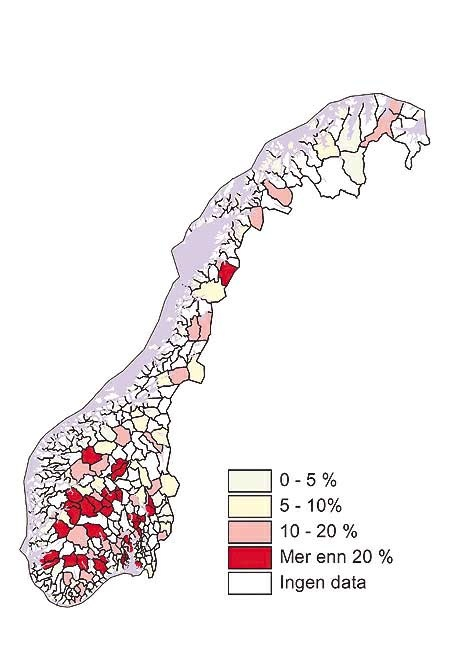
\includegraphics[width=90mm]{straleskart.jpg}
\caption{Oversiktskart. Prosenttallene angir hvor mange prosent over den anbefalte grensen på $200Bq/m^3$ det er funnet i boliger i disse områdene.
\textit{Kilde: Statens strålevern}
}
\label{fig:oversiktskart}
\end{figure}

\begin{figure}[ht!]
    \begin{center}
    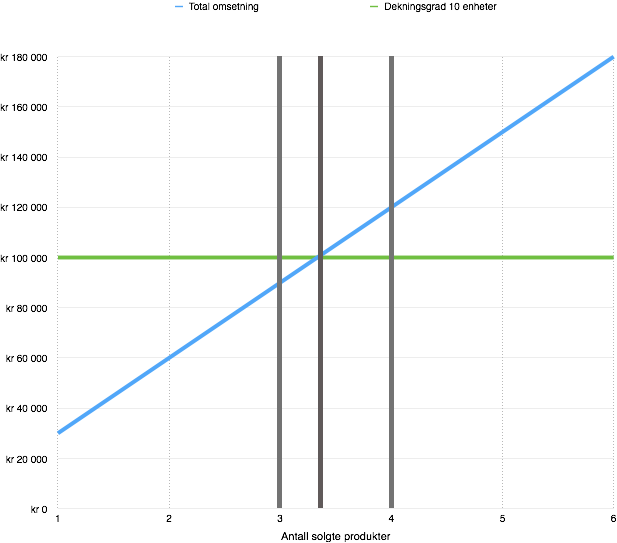
\includegraphics[width=0.9\textwidth]{graph.png}
    \caption{Profitabelhet for radonmåleren. Grønn linje er kostnad for 10 enheter. Blå er total omsetning per enhet}
    \label{fig:profitmargin}
    \end{center}
\end{figure}


\end{alphasection}

\end{document}
